The FEM panel is intended to present users with a selection of FEM
applications that will take a building model generated by the BIM
application and the EVENT from the event application and perform a
deterministic simulation.  At present there is only one application
available, OpenSees and there is no application selection box.  That
will be modified in future versionsto allow user to provide their own
simulation application.  This is not the standard OpenSees executable,
but consists of a pre- and post-processor to take the BIM and EVENT
file and use OpenSees to determine the response, returning these
responses in an EDP.

For the OpenSees application the user is required to specify the
options to be used in the transient analysis. As shown \Cref{fig:fem},
this includes the choice of
\begin{enumerate}
\item Solution algorithm, the default is Newton Raphson.
\item Integration Scheme, the default is Newmarks linear acceleration
  method.
\item Convergence Test, the default is a norm on the unbalance force.
\item Convergence tolerance
\item Damping Ratio.
\end{enumerate}

\begin{figure}[!htbp]
  \centering {
    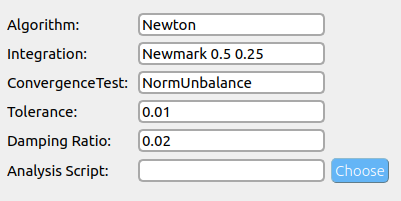
\includegraphics[width=0.8\textwidth]
    {usage/figures/fem.png} }
  \caption{Options for \texttt{OpenSees} transient analysis}
  \label{fig:fem}
\end{figure}

All the options available can be found in the OpenSees online user
manual.\\

A default transient analysis script is run with these inputs. It is
built for Version 3.0.0+ of OpenSees and uses a divide and conquer
algorithm in event of a convergence failure issue. This new algorithm
does not always work. \\

The user is also able to specify their own analysis script to run
instead of the default. When chosen the variables numStep and dt that
are obtained from the EVENT are set by the program. These variables
can be used by the user when providing their own analysis script.
